\section{Evolutionary Algorithm}

\begin{frame}{Search}
  \begin{columns}
  \column{0.5\textwidth}
  \centering
   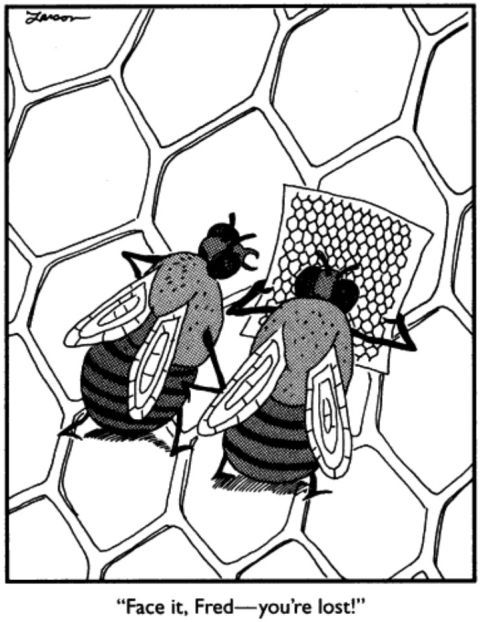
\includegraphics[height=\textwidth]{img/farside}
   \column{0.5\textwidth}
   \begin{itemize}
      \item \alert{common scenario:} you can recognize a good solution, but you don't know how to find one
      \item encountered by computer scientists (and everyone else, too)
      \item \alert{common approach:} try different options, evaluate outcomes to help choose next options to try
       \item this is called \alert{search}    
       \end{itemize}
   \end{columns}
\end{frame}

\begin{frame}{Evolutionary Algorithm: Vocabulary}

\begin{columns}
\begin{column}{0.25\textwidth}
\begin{itemize}
  \item individual
  \item population
  \item fitness
  \item genotype
  \item phenotype
  \item mutation
\end{itemize}
\end{column}
\begin{column}{0.75\textwidth}
\begin{figure}
    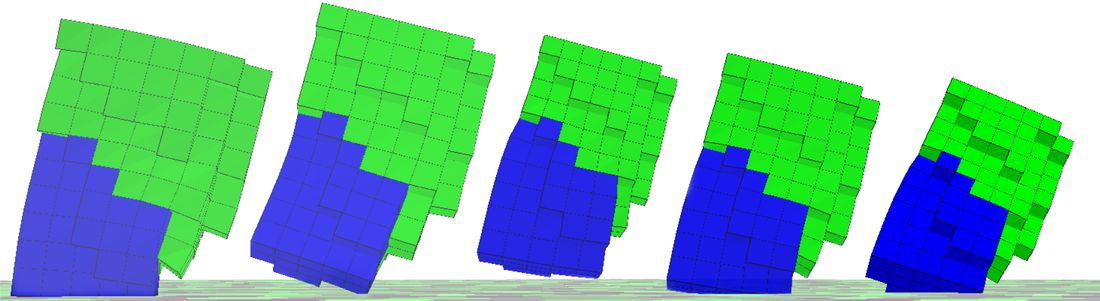
\includegraphics[width=\textwidth]{img/jumpertimeseries3_orig} \\
  \vspace{1ex}
  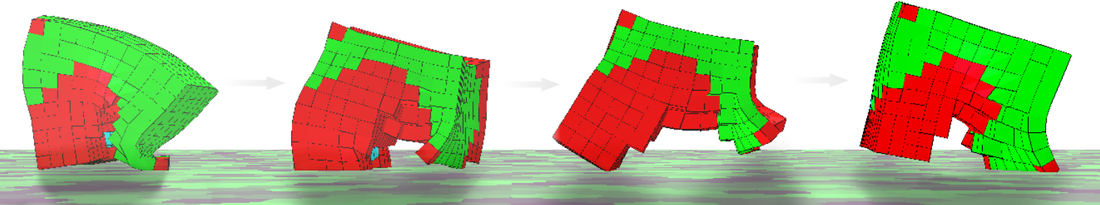
\includegraphics[width=\textwidth]{img/runnershortarrow_orig}
  \captionsetup{singlelinecheck=off,justification=raggedright}
  \caption{Illustrative examples of candidate solutions in an evolutionary algorithm \cite[Figures 1, 12]{Cheney2013UnshacklingEncoding}.}
\end{figure}
\end{column}
\end{columns}
    
\end{frame}

\begin{frame}{Evolutionary Algorithm: Overview}

\begin{figure}
  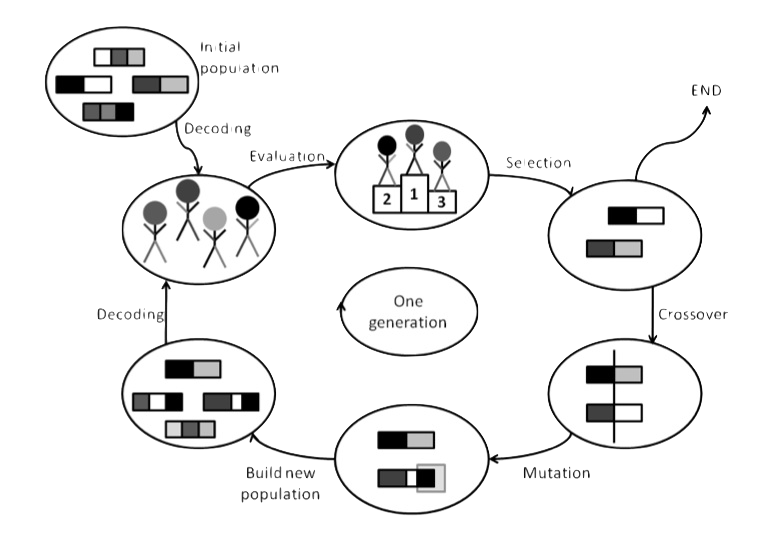
\includegraphics[width=0.8\textwidth]{img/working_principle_of_EA}
  \captionsetup{singlelinecheck=off,justification=raggedright}
  \caption{A schematic illustration of the evolutionary algorithm \cite[Figure 1]{Prothmann2009EvolutionaryOptimisation}.}
\end{figure}
    
\end{frame}


\begin{frame}{Evolutionary Algorithm: Example}
\begin{figure}
  \includemedia[width=\linewidth,height=0.6\textwidth, flashvars={scaleMode=zoom}]{}{http://www.youtube.com/v/z9ptOeByLA4?t=1m08s&amp;rel=0&amp;showinfo=0}
  \captionsetup{singlelinecheck=off,justification=raggedright}
\href{https://youtu.be/z9ptOeByLA4?t=1m08s}{\caption{Evolution in Action \cite{Cheney2013UnshacklingEncoding}}}
\end{figure}
\end{frame}

\begin{frame}{Evolutionary Algorithm: Problem Statement}
  
  \begin{columns}
\begin{column}{0.6\textwidth}
 What makes an evolutionary algorithm work?
\end{column}
\begin{column}{0.4\textwidth}
\begin{center}
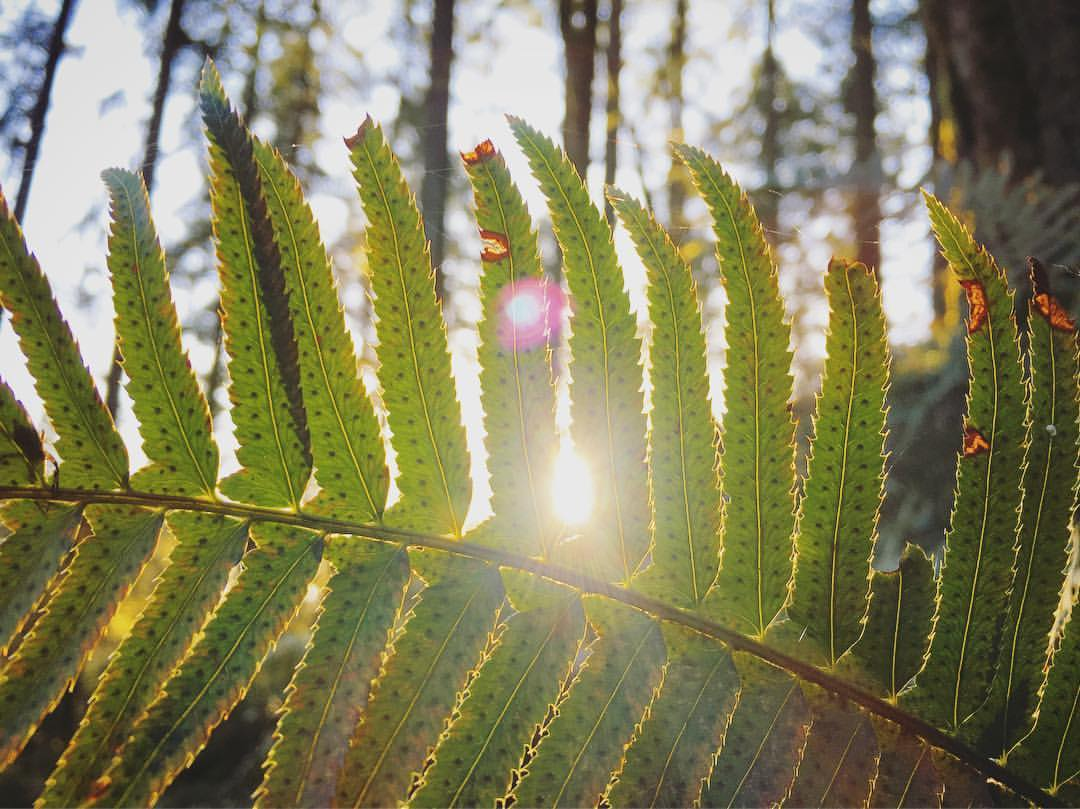
\includegraphics[width=\textwidth,trim={7cm 0 13cm 0},clip]{img/sunfern}
\end{center}
\end{column}
\end{columns}
 
\end{frame}